
%%%%%%%%%%%%%%%%%%%%%%% file typeinst.tex %%%%%%%%%%%%%%%%%%%%%%%%%
%
% This is the LaTeX source for the instructions to authors using
% the LaTeX document class 'llncs.cls' for contributions to
% the Lecture Notes in Computer Sciences series.
% http://www.springer.com/lncs       Springer Heidelberg 2006/05/04
%
% It may be used as a template for your own input - copy it
% to a new file with a new name and use it as the basis
% for your article.
%
% NB: the document class 'llncs' has its own and detailed documentation, see
% ftp://ftp.springer.de/data/pubftp/pub/tex/latex/llncs/latex2e/llncsdoc.pdf
%
%%%%%%%%%%%%%%%%%%%%%%%%%%%%%%%%%%%%%%%%%%%%%%%%%%%%%%%%%%%%%%%%%%%


\documentclass[runningheads,a4paper]{llncs}

\usepackage{amssymb}
\setcounter{tocdepth}{3}
\usepackage{graphicx}
\usepackage{amssymb,amsmath,array}

\usepackage{url}
\urldef{\mailsa}\path|{alfred.hofmann, ursula.barth, ingrid.haas, frank.holzwarth,|
\urldef{\mailsb}\path|anna.kramer, leonie.kunz, christine.reiss, nicole.sator,|
\urldef{\mailsc}\path|erika.siebert-cole, peter.strasser, lncs}@springer.com|
\newcommand{\keywords}[1]{\par\addvspace\baselineskip
\noindent\keywordname\enspace\ignorespaces#1}

\begin{document}

\mainmatter  % start of an individual contribution

% first the title is needed
\title{Joint Neighborhood Subgraphs Link Prediction}

% a short form should be given in case it is too long for the running head
%\titlerunning{Lecture Notes in Computer Science: Authors' Instructions}

% the name(s) of the author(s) follow(s) next
%
% NB: Chinese authors should write their first names(s) in front of
% their surnames. This ensures that the names appear correctly in
% the running heads and the author index.
%
\author{Dinh Tran-Van$^1$ \and Alessandro Sperduti$^1$ \and Fabrizio Costa$^2$}
%
\authorrunning{Dinh Tran-Van, Alessandro Sperduti, and Fabrizio Costa$^2$}
% (feature abused for this document to repeat the title also on left hand pages)

% the affiliations are given next; don't give your e-mail address
% unless you accept that it will be published
\institute{$^1$ Department of Mathematics, Padova University, Italy\\
%via Trieste, 63, 35121 Padova, Italy\\
$^2$ Department of Computer Science, University of Exeter, United Kingdom\\ 
$\lbrace$dinh, sperduti$\rbrace$@math.unipd.it, f.costa@exeter.ac.uk
%\mailsc\\
}
%\url{http://www.springer.com/lncs}}

%
% NB: a more complex sample for affiliations and the mapping to the
% corresponding authors can be found in the file "llncs.dem"
% (search for the string "\mainmatter" where a contribution starts).
% "llncs.dem" accompanies the document class "llncs.cls".
%

\toctitle{Lecture Notes in Computer Science}
\tocauthor{Authors' Instructions}
\maketitle


\begin{abstract}
A crucial computational task for relational and network data is the ``link prediction problem'' which allows for example to discover unknown interactions between proteins to explain the mechanism of a disease in biological networks, or to suggest novel products for a customer in a e-commerce recommendation system. Most link prediction approaches however do not effectively exploit the contextual information available in the neighborhood of each edge. Here we propose to cast the problem as a binary classification task over the union of the pair of subgraphs located at the endpoints of each edge. We model the classification task using a support vector machine endowed with an efficient graph kernel and achieve state-of-the-art results on several benchmark datasets. 

\keywords{Link prediction, graph kernels}
\end{abstract}

\section{Introduction and related work}
We are witnessing a constant increase of the rate at which data is being produced and made available in machine readable formats. Interestingly it is not only the quantity of data that is increasing, but also its complexity, i.e. not only are we measuring a number of attributes or features for each data point, but we are also capturing their mutual relationships, that is, we are considering non independent and identically distributed (non i.i.d.) data. This yields collections that are best represented as graphs or relational data bases and requires a more complex form of analysis. As cursory examples of application domains that are social networks, where nodes are people and edges encode a type of association such as friendship or co-authorship, bioinformatics, where nodes are proteins and metabolites and edges represent a type of chemical interaction such as catalysis or signaling, and e-commerce, where nodes are people and goods and edges encode a ``buy'' or ``like'' relationship.
A key characteristic of this type of data collections is the sparseness and dynamic nature, i.e. the fact that the number of recorded relations is significantly smaller than the number of all possible pairwise relations, and the fact that these relations evolve in time. A crucial computational task is then the ``link prediction problem'' which allows to suggest friends, or possible collaborators for scientists in social networks, or to discover unknown interactions between proteins to explain the mechanism of a disease in biological networks, or to suggest novel products to be bought to a customer in a e-commerce recommendation system. Many approaches to link prediction that exist in literature can be partitioned according to \textit{i}) whether additional or ``side'' information is available for nodes and edges or rather only the network topology is considered and \textit{ii}) whether the approach is unsupervised or supervised. 

Unsupervised methods are non-adaptive (i.e. they do not have parameters that are tuned on the specific problem instance), and can therefore be computationally efficient. In general they define a score for any node pair that is proportional to the existence likelihood of an edge between the two nodes. \textit{Adamic-Adar} \cite{adamic} computes the weighted sum over the common neighbors where the weight is inversely proportional to the (log of) each neighbor node degree. The \textit{preferential attachment} method computes a score simply as the product of the node degrees in an attempt to exploit the ``rich get richer'' property of certain network dynamics. \textit{Katz} \cite{katz} takes into account the number of common paths with different lengths between two nodes, assigning more weight to shorter paths. The \textit{Leicht-Holme-Newman} method \cite{lhni} computes the number of intermediate nodes. In \cite{matrix-factorization} the score is derived from the singular value decomposition of the adjacency matrix. 

Supervised link prediction methods convert the problem into a binary classification task where links present in the network (at a given time) are considered as positive instances and a subset of all the non links are considered as negative instances. Following \cite{matrix-factorization}, we can further group these methods into four classes: feature-based models, graph regularization models, latent class models and latent feature models. 
A Bayesian nonparametric approach is used in \cite{nonparametric} to compute a nonparametric latent feature model that does not need a user defined number of latent features but rather induces it as part of the training phase. 
In \cite{matrix-factorization} a matrix factorization approach is used to extract latent features that can take into consideration the output of an arbitrary unsupervised method. The authors show a significant increase in predictive performance when considering a ranking loss function suitable for  the imbalance problem, i.e. when the number of negative is much larger than the number of positive instances. 

In general supervised methods exhibit better accuracies compared to unsupervised methods although incurring in much higher computational and memory complexity costs.
Moreover, most approaches implicitly represent the link prediction problem and the inference used to tackle it as a disjunction over the edges, that is, information on edges is propagated in such a fashion so that for a node to have $k$ neighbors or $k+1$ does not make a drastic difference.
We claim that this hypothesis is likely putting a cap on the discriminative power of classifiers and therefore we propose a novel supervised method that employs a conjunctive representation. We call the method ``joint neighborhood subgraphs link prediction'' (JNSL). The key idea here is to transform the link prediction task into a binary classification on suitable small subgraphs which we then solve using an efficient graph kernel method.


\section{Method}

\subsection{Definitions and notation}
We represent a problem instance as a graph $G=(V,E)$ where $V$ is the set of nodes and $E$ is the set of links. The set $E$ is partitioned into the subset of observed links ($O$) and the subset of unobserved links ($U$). Like other approaches we assume that all un-observed links are indeed ``non-links'' and we therefore define the link prediction problem as the task of ranking candidate links from the most to the least probable to recover links in $O$ but not in $U$ exploiting only the network topology.


We define the \textit{distance} $\mathcal{D}(u,v)$ between two nodes $u$ and $v$, as the number of edges on the shortest path between them. The \textit{neighborhood} of a node $u$ with radius $r$, $N_r(u) = \lbrace v\ |\ \mathcal{D}(u,v) \leq r \rbrace$, is the set of nodes at distance no greater than $r$ from $u$. The corresponding \textit{neighborhood subgraph} $\mathcal{N}_{r}^{u}$ is the  subgraph induced by the neighborhood (i.e. considering all the edges with endpoints in $N_r(u)$). The \textit{degree} of a node $u$, $d(u) = |\mathcal{N}_{1}^{u}|$, is the cardinality of its neighborhood. The maximum node degree in the graph $G$ is $d(G)$.



\subsection{Link encoding as subgraphs union}
\label{sec:link}
Most methods for link prediction compute pairwise nodes similarities treating  the nodes defining the candidate edge independently. Instead we propose to jointly consider both candidate endpoint nodes together with their extended ``context''. To do so we build a graph starting from the two nodes and the underlying network. Given nodes $u$ and $v$, we first extract the two neighborhood sets with a user defined radius $R$ rooted at $u$ and $v$ to obtain $N_R(u)$ and $N_R(v)$, respectively. We then consider the graph $\mathcal{J}$ induced by the set union $N_R(u) \cup N_R(u)$. Finally we add an auxiliary node $w$ and the necessary edges to connect it to $u$ and $v$ (see Fig.\ref{fig:example}).

\begin{figure}
\centering
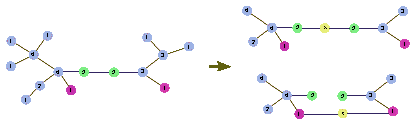
\includegraphics[width=.9\textwidth]{subgraphs}
\caption{Left) We represent with solid lines edges belonging to the training material and with a dotted line edges belonging to the test material. Right) joint neighborhood subgraphs for an existing (green endpoints) (top) and a non existing (red endpoints) link (bottom). These graphs will receive respectively a positive and a negative target.}
\label{fig:example}
\end{figure}


\subsection{Node labeling}
We propose to use a graph kernel approach to classify the subgraphs encoding each link. In our setup nodes are not endowed with any ``side'' information. However to increase the discriminative power of the similarity notion induced by the graph kernel, instead of assuming a dummy, non-informative label on each node, we propose to use a node labeling function $\ell$ which assigns as the discrete label the node degree. More precisely, for nodes having degree less than or equal than a user defined threshold $T$ ($T=5$ in our experimental evaluation) we use as label the degree value. Degree values larger than $T$ are subsequently discretized into $k$ levels. Here the implicit assumption is that nodes with similar degrees have common properties. Formally, the labeling function is defined as:
\begin{center}
$\ell(u) = \left\{
	\begin{array}{ll}
		d(u),\  & \mbox{if } d(u) \leq T \\
		T+i,\ & \mbox{if } d(u) > T
	\end{array}
\right.$,
\end{center}
where $i = \lceil \frac{d(u)-T}{bin}\rceil$, $bin = \frac{d(G)-T}{\lambda - T}$ and $\lambda$ ($\lambda > T$) is the maximum number of symbols used. The value of $\lambda$ depends on the degree distribution and can be tuned as a hyperparameter of the approach.



\subsection{The graph kernel}
Here we briefly describe an efficient graph kernel called the Neighborhood Subgraph Pairs Distance kernel (NSPDK) introduced in \cite{nspdk}. NSPDK is an instance of ``decompositional'' kernels \cite{convolution-kernel} based on the idea of counting the number of common small subgraphs between two graphs. The subgraphs are pairs of neighborhoods whose roots are at a short distance. 

Given a labeled graph $G \in \mathcal{G}$ and two rooted graphs $A_u, B_v$, we first define the relation $R_{r,d}(A_u, B_v, G)$ to be true {\em iff} $A_u \cong \mathcal{N}_r^u$ is (up to isomorphism $\cong$) a neighborhood subgraph with radius $r$ of $G$ and so is $B_v \cong  \mathcal{N}_r^v$, such that $v$ is a distance $d$ from $u$: $\mathcal{D}(u,v)= d$. We then define the inverse relation $R^{-1}$ that returns all pairs of neighborhoods of radius $r$ at distance $d$ in $G$, $R^{-1}_{r,d}(G) = \lbrace A_u, B_v | R_{r,d}(A_u,B_v,G)=true\rbrace$. The kernel $\kappa_{r,d}$ over $\mathcal{G} \times \mathcal{G}$ is the number of such fragments in common in two input graphs:
\begin{center}
$\kappa_{r,d}(G,G^{'}) = 
\!\!\!\!\!\!\!\!\!\!\!\! 
\sum\limits_{\substack{A_u, B_v \ \in \ R_{r,d}^{-1}(G) \\ 
{A'}_{u'}, {B'}_{v'} \ \in \ R_{r,d}^{-1}(G')
}} \!\!\!\!\!\!\!\!\!\!\!\!  { { \textbf{1}_{A_{u} \cong A'_{u'}}} \cdot {
\textbf{1}_{B_{v} \cong B'_{v'}}} }$, 
\end{center}
\noindent where $\textbf{1}_{A \cong B}$ is the \textit{exact matching function} that returns 1 if $A$ is isomorphic to $B$ and 0 otherwise. Finally, the NSPDK is defined as $K(G,G') = \sum\limits_{r}{\sum\limits_{d}{\kappa_{r,d}(G,G')}}$, where for efficiency reasons, the values of $r$ and $d$ are upper bounded to a given maximal $r^*$ and $d^*$, respectively.

% Related to exact matching function, this function needs to solve the graph isomorphism problem. This problem is not known to be solvable in polynomial time nor to be NP-complete. In \cite{nspdk}, they propose an approximate method to figure out graph isomorphism problem. It first transforms graphs into strings. It then employ a hash function to map each unique string with an integer number. Finally, two graphs are isomorphic if they have the same corresponding integer numbers.

\subsection{Joint neighborhood subgraphs link prediction}

In the link prediction problem we are given a graph $G(V,E)$ and a binary target vector $Y=\{y_{(0,0)},y_{(0,1)}, \cdots, y_{(|V|,|V|)}\}$ where $y_{(u,v)}=1$ if $(u,v) \in E$ and 0 otherwise. The training data is obtained considering a random subset of edges in $E^{tr} \in E$ and inducing a training graph $G^{tr}=(V,E^{tr})$. Note that the graph used for training does not contain any of the edges that will be queried in the test phase. The remaining edges $E^{ts} = E \setminus E^{tr}$ are used to partition the target vectors: $Y^{tr} = \{y_{(u,v)} | (u,v) \in E^{tr}\}$, $Y^{ts} = \{y_{(u,v)} | (u,v) \in E^{ts}\}$.
We can now cast the problem as a standard classification problem in the domain of graphs. Given $G^{tr}$ we build a train and test set as the corresponding joint neighborhood subgraphs as detailed in Section~\ref{sec:link}. 
We can now compute a Gram matrix of the instances and solve the classification task using for example the efficient LinearSVC library \cite{svm}.

\section{Empirical evaluation}
To compare the performance of the JNSL method with other link prediction approaches we follow \cite{matrix-factorization} and use 6 datasets belonging to different domains.
\begin{itemize}
\item \textit{Protein }\cite{protein-protein}: nodes are proteins and edges encodes a thresholded interaction confidence between proteins. It has 2617 nodes and 11855 links with an average degree of 9.1.

\item \textit{Metabolic} \cite{metabolic}: nodes are enzyme and metabolites, edges are present if the enzyme catalyzes for a reaction that include those chemical compounds. It has 668 nodes and 2782 links with an average degree of 8.3.

\item \textit{Nips} \cite{nips}: nodes are authors at the NIPS conference from the first to the $12^{th}$ edition. Links encode the co-authorhip relation, i.e. if two authors have published a paper together. This network contains 2865 nodes and 4733 links with an average degree of 3.3.

\item \textit{Condmat} \cite{condmat}: nodes are scientists working in condensed matter physics, edges encode co-authorship. This network has 14230 nodes and 1196 links with an average degree of 0.17.

\item \textit{Conflict} \cite{conflict1}, \cite{conflict2}: nodes are countries and edges encode a conflict or a dispute. We have 130 nodes and 180 links in total in this network with an average degree of 2.5.

\item \textit{Powergrid} cite{powergrid}: a network of electric powergrid in US. It has 4941 nodes and 6594 links. The average degree is 2.7.
\end{itemize}

We evaluate the performance of employed methods by splitting 10 times the data in a train and a test part. For \textit{Protein}, \textit{Metabolic}, \textit{Nips} and \textit{Conflict} networks, we use 10$\%$ of the edges to induce the training set while for \textit{Condmat} and \textit{Powergrid} we use 90$\%$ of the links. The performance of each method is computed as the average of the AUC-ROC over the 10 rounds.

\textbf{Model Selection}: The values of different hyper-parameters are set by using a 3-fold on the training set, that is, always considering only the training network, we use one fold for fitting the parameters and the rest two folds for validating the effect of the hyper parameter choice. We tune the values of radius for extracting subgraphs $R$ in $\lbrace 1, 2 \rbrace$, $\lambda$ in node label function in $\lbrace 10, 15 \rbrace$, for $r$ and $d$ parameters of NSPDK in $\lbrace  1, 2 \rbrace$ and $\lbrace  1, 2, 3 \rbrace$, respectively. Finally, the regularization tradeoff $C$ for the SVM is picked up in $\lbrace 10^{-4}, 10^{-3}, 10^{-2},\ 10^{-1}, 1,\ 10,\ 10^2, 10^3,\ 10^4 \rbrace$.

\section{Results and discussion}
In Table \ref{result_table}, we report the performance of link prediction methods measured as the AUC-ROC value on 6 datasets. From the results on the table, we can group methods into two groups based on their performances: supervised methods and unsupervised methods. The performance of supervised methods are considerably higher than unsuperivsed ones in most cases, except in the Conflict dataset where Sup-Top outperforms Fact+Scores, but with a very small difference. Concerning supervised methods, JNSL outperforms Fact-Scores in all cases. The difference between their performance is small in PowerGrid and Protein datasets with 0.5$\%$ and 0.8$\%$, respectively. And the big gap is in the Condmat dataset with 7.4$\%$. 

\begin{table}
\caption{AUC-ROC performance on 6 datasets. Legend: AA: Adamic-Adar, PA \cite{pa} preferential Attachment, SHP: Shortest Path, Sup-Top \cite{matrix-factorization}: Liear regression running on unsupervised scores, SVD \cite{matrix-factorization}: Singular value decomposition, Fact+Scores \cite{matrix-factorization}: Factorization with unsupervised scores, JNSL: joint neighborhood subgraph link (our method). In bold the highest score.}
\centering
\setlength{\tabcolsep}{1mm}
\begin{tabular}{|c|c|c|c|c|c|c|}

\hline
         & \multicolumn{6}{c|}{\textbf{Datasets}}\\
 \hline
\textbf{Methods} & Protein & Metabolic & Nips & Condmat & Conflict & PowerGrid\\
	& ($\%$) & ($\%$) & ($\%$) & ($\%$) & ($\%$) & ($\%$)\\
\hline
AA & 56.4$\pm$0.5 & 52.4$\pm$0.5 & 51.2$\pm$0.2 & 56.7$\pm$1.4 & 50.7$\pm$0.8 & 58.9$\pm$0.3\\
PA & 75.0$\pm$0.3 & 52.4$\pm$0.5 & 54.3$\pm$0.5 & 71.6$\pm$2.6 & 54.6$\pm$2.4 & 44.2$\pm$01.0\\
SHP & 72.6$\pm$0.5 & 62.6$\pm$0.4 & 51.7$\pm$0.3 & 67.3$\pm$1.8 & 51.2$\pm$1.4 & 65.9$\pm$1.5\\
Katz & 72.7$\pm$0.5 & 60.8$\pm$0.7 & 51.7$\pm$0.3 & 67.3$\pm$1.7 & 51.2$\pm$1.4 & 65.5$\pm$1.6 \\
Sup-Top & 75.4$\pm$0.3 & 62.8$\pm$0.1 & 54.2$\pm$0.7 & 72.0$\pm$2.0 & 69.5$\pm$7.6 & 70.8$\pm$6.2\\
SVD & 63.5$\pm$0.3 & 53.8$\pm$1.7 & 51.2$\pm$3.1 & 62.9$\pm$5.1 & 54.1$\pm$9.4 & 69.1$\pm$2.6\\
Fact+Scores & 79.3$\pm$0.5 & 69.6$\pm$0.2 & 61.3$\pm$1.9 & 81.2$\pm$2.0 & 68.9$\pm$4.2 & 75.1$\pm$2.0 \\
JNSL & \textbf{80.1$\pm$0.8} & \textbf{72.5$\pm$0.7} & \textbf{62.1$\pm$0.8} & \textbf{88.6$\pm$2.3} & \textbf{72.0$\pm$0.9} & \textbf{75.6$\pm$0.7} \\
 \hline 
\end{tabular}
\label{result_table}
\end{table}

\section{Conclusion and future work}
We have presented a novel approach to link prediction in absence of side information that can effectively exploit the topological contextual information available in the neighborhood of each edge. We have empirically shown that this approach achieves very competitive results compared to other state-of-the-art methods.
In future work, we will investigate how to make use of multiple and heterogeneous information sources when these are available for nodes and edges.

\begin{thebibliography}{4}

\bibitem{adamic} Adamic, L.A., and Eytan, A.: Friends and neighbors on the web. Social networks 25.3 (2003): 211-230.

\bibitem{katz} Katz, L.: A new status index derived from sociometric analysis. Psychometrika 18.1 (1953): 39-43.

\bibitem{lhni} Leicht, E.A., et al.: Vertex similarity in networks. Physical Review E 73.2 (2006): 026120.

\bibitem{pa}  Barabasi, A.L, Albert, R.: Emergence of Scaling in Random Networks, Science 286 (1999) 509.

\bibitem{matrix-factorization} Menon, A., and Charles, E.: Link prediction via matrix factorization. Machine Learning and Knowledge Discovery in Databases (2011): 437-452.

\bibitem{nonparametric} Miller, K., Michael, et al.: Nonparametric latent feature models for link prediction. Advances in neural information processing systems. 2009.

\bibitem{protein-protein} Von. M.C, et al.: Comparative assessment of large-scale data sets of protein–protein interactions. Nature 417.6887 (2002): 399-403.

\bibitem{metabolic} Yamanishi, Y., et al.: Supervised enzyme network inference from the integration of genomic data and chemical information. Bioinformatics 21.suppl-1 (2005): i468-i477.

\bibitem{nips} Rowies, S.: NIPS dataset (2002), http://www.cs.nyu.edu/~rwoeis/data.html

\bibitem{condmat} Lichtenwalter, R. N., et al.: New perspectives and methods in link prediction. Proceedings of the 16th ACM SIGKDD international conference on Knowledge discovery and data mining. ACM, 2010.

\bibitem{conflict1} Ghosn, F., et al.: The MID3 data set, 1993–2001: Procedures, coding rules, and description. Conflict Management and Peace Science 21.2 (2004): 133-154.

\bibitem{conflict2} Ward, M.D., et al.: Disputes, democracies, and dependencies: A reexamination of the Kantian peace. American Journal of Political Science 51.3 (2007): 583-601.

\bibitem{powergrid} Watts, D.J., and Steven, H.S.: Collective dynamics of ‘small-world’networks. nature 393.6684 (1998): 440-442.

\bibitem{nspdk} Costa, F, and Kurt, D.G.: Fast neighborhood subgraph pairwise distance kernel. Proceedings of the 26th International Conference on Machine Learning. Omnipress, 2010.

\bibitem{convolution-kernel} Haussler, D.: Convolution kernels on discrete structures. Vol. 646. Technical report, Department of Computer Science, University of California at Santa Cruz, 1999.

\bibitem{svm} http://www.scikit-learn.org/

%\bibitem{jour} Smith, T.F., Waterman, M.S.: Identification of Common Molecular
%Subsequences. J. Mol. Biol. 147, 195--197 (1981)
%
%\bibitem{lncschap} May, P., Ehrlich, H.C., Steinke, T.: ZIB Structure Prediction Pipeline:
%Composing a Complex Biological Workflow through Web Services. In: Nagel,
%W.E., Walter, W.V., Lehner, W. (eds.) Euro-Par 2006. LNCS, vol. 4128,
%pp. 1148--1158. Springer, Heidelberg (2006)
%
%\bibitem{book} Foster, I., Kesselman, C.: The Grid: Blueprint for a New Computing
%Infrastructure. Morgan Kaufmann, San Francisco (1999)
%
%\bibitem{proceeding1} Czajkowski, K., Fitzgerald, S., Foster, I., Kesselman, C.: Grid
%Information Services for Distributed Resource Sharing. In: 10th IEEE
%International Symposium on High Performance Distributed Computing, pp.
%181--184. IEEE Press, New York (2001)
%
%\bibitem{proceeding2} Foster, I., Kesselman, C., Nick, J., Tuecke, S.: The Physiology of the
%Grid: an Open Grid Services Architecture for Distributed Systems
%Integration. Technical report, Global Grid Forum (2002)
%
%\bibitem{url} National Center for Biotechnology Information, \url{http://www.ncbi.nlm.nih.gov}

\end{thebibliography}

\end{document}
